% Comments are written after a percent symbol. They are not compiled (i.e. written to the PDF).
% See appendix 1 for a list of options for the xamk document class
\documentclass[minted, listings, pgfplots, bib]{xamk} % Use the xamk.cls document class
\addbibresource{main.bib} % Add your bibliography BibTeX file with this command
\addbibresource{extra.bib} % Extra references to provide examples for various entry types

% Anything meant to be written to the PDF must be within the document environment.
\begin{document}
    %\embedfile{./attach.zip} % Attach attach.zip file to output PDF
    
    % Choose one of the following two title page formats. See appendix 1 for more information.
    
    % Format for title page of assignment/report/etc.
    %\xamkstudent{John Smith}{1234567}{ITMI17SP}
    %\xamkstudent{Jane Smith}{1234568}{ITMI17SP} % More than 1 student can be listed
    %\xamkstudent{Jake Smith}{1234569}{ITMI17SP} % The only limit is page space
    %\xamkpapertitle{Assignment 3}
    %\xamkpapersubtitle{Doing The Thing} % Optional
    %\xamkpapertype{Assignment}
    %\xamkcoursename{Computer Hardware}
    %\xamkpaperdate{2020}
    \maketitle % Creates title page with the preceding options
    
    % Format for title page of thesis.
    %\xamkstudentname{John Smith}
    %\xamkpapertitle{This And That And The Other Thing}
    %\xamkpapersubtitle{Doing The Thing} % Optional
    %\xamkdegreetype{Master's Degree} % Optional, defaults to "Bachelor's Degree"
    %\xamkdegreeprogramme{Bachelor of Engineering}
    %\xamkpaperdate{2020}
    %\maketitle[thesis] % Creates thesis title page with preceding options
    
    % Format for the thesis abstract page (some info copied from thesis title page).
    %\xamkpagecount{99} % Number of pages (not including appendices)
    %\xamkappendixpagecount{9} % Number of appendix pages
    %\xamkthesiscommissioner{Random Company Ltd.}
    %\xamkthesissupervisor{Bob Smith}
    %\xamkthesiskeywords{documentation, model, thesis, report writing}
    %\xamkthesisabstractfile{thesis-abstract.tex} % Takes name of .tex file containing abstract
    %\makethesisabstract % Creates thesis abstract page with preceding options
    
    \tableofcontents % Automatically generates table of contents, based on sections/subsections/etc.
    
    % tex files can be imported with \input{} or \include{}
    % \input{} just imports the file, while \include{} also ensures page breaks before and after
    \input{chapter1} % Imports chapter1.tex from the same directory as xamk-template.tex
    \section{Some Examples}

\subsection{Tables}

Notice the missing | and \verb|\hline| in the \verb|chapter2.tex| file and their effects.

% If you don't need a caption/label you can remove the table environment.
\begin{table}[H]
    %\centering
    % Table captions should go above their tables, according to the official styling
    \caption{An example table} % \citecaption can also be used in tables
    \label{tab:tabletest}
    % extra | before first l and missing | after the last l
    \begin{tabular}[b]{ || l | l  }
    	\hline % "\\" adds a linebreak, "\hline" adds a horizontal line
    	Measurement 1 & $(20.49 \pm 0.01)\si{mm}$ \\\hline
    	Measurement 2 & $(20.47 \pm 0.01)\si{mm}$ \\%\hline
    	Measurement 3 & $(18.63 \pm 0.01)\si{mm}$ \\\hline
    \end{tabular}
\end{table}

\subsection{Mathematics}

% For physics units, \si{} can be used to distinguish units from variables (variables are italic).
% The "&"s control alignment. Try moving them around to adjust alignment.
\begin{align*}
    % _{} is used for subscript, ^{} is used for superscript
	V_{cuboid} &= w h l = 20.49\si{mm} \times 20.47\si{mm} \times 18.63\si{mm} \approx 7814\si{mm^{3}} \\ 
	% Notice how this \num{} converts its input into scientific notation
	G &= \num{6.673e-11}\si{N.m^{2}.kg^{-2}} \\ 
	% \num{} can also add those small spaces in large/small numbers
	\num{1000000} &= \num{1000000000000} \times \num{0.000001} \\
	% Calculus
	x &= \frac{-b \pm \sqrt{b^2 - 4ac}}{2a} \\
	\int_{x^2 + y^2 \leq R^2} & f(x,y)\,dx\,dy
	    = \int_{\theta=0}^{2\pi} \int_{r=0}^R f(r\cos\theta,r\sin\theta) r\,dr\,d\theta. \\
    % Matrices ("&" doesn't control alignment from within the matrix environment)
    \begin{bmatrix} 1 & 2 & 3 \\ 4 & 5 & 6 \end{bmatrix}&
        \begin{bmatrix} 7 & 8 \\ 9 & 10 \\ 11 & 12 \end{bmatrix} =
        \begin{bmatrix} 58 & 64 \\ 139 & 154 \end{bmatrix}
	% If \\ was included after the last row it'd create an extra empty line of space below
\end{align*}
% Empty lines should be avoided around an align* environment, to preserve page space.
% Alternatively, a comment (even a "%" by itself) can be used.

\subsection{Graphics}

It's a cube with a hole through the top. Try changing the value of \texttt{cubex}.

% If you don't need the caption/label you can remove the figure environment.
\begin{figure}[H]
    %\centering
    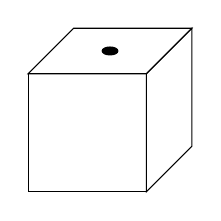
\begin{tikzpicture}
        \pgfmathsetmacro\cubex{1.5}
        \pgfmathsetmacro\cubey{1.5}
        \pgfmathsetmacro\cubez{1.5}
        \draw (0,0,0) -- ++(-\cubex,0,0) -- ++(0,-\cubey,0) -- ++(\cubex,0,0) -- cycle;
        \draw (0,0,0) -- ++(0,0,-\cubez) -- ++(0,-\cubey,0) -- ++(0,0,\cubez) -- cycle;
        \draw (0,0,0) -- ++(-\cubex,0,0) -- ++(0,0,-\cubez) -- ++(\cubex,0,0) -- cycle;
        \pgfmathsetmacro\circlex{\cubex/2}
        \pgfmathsetmacro\circlez{\cubez/2}
        \draw[fill=black] (-\circlex,0,-\circlez) ellipse (0.1 and 0.05);
    \end{tikzpicture}
    \citecaption{cube}{A cube drawn with TikZ} % 1st argument is the citation key, 2nd is the caption
    \label{fig:cube}
\end{figure}

\subsection{Graphs}

% If you don't need the caption/label you can remove the figure environment.
\begin{figure}[H]
    %\centering
    \begin{tikzpicture}
    % Google "pgfplots gallery" to see examples of graphs and how to make them.
    % If you need negative numbers, add the "axis lines=middle" option to axis.
    \begin{axis}[
    xmin=0, xmax=1.2, ymin=0, ymax=2, % sets x-axis and y-axis limits
    xlabel={foo $a_1$ (\si{m.s^{-2}})}, % set x axis label
    ylabel={bar \\ $a_2$ (\si{m.s^{-2}})}] % set y axis label
    	\addplot+[only marks,error bars/.cd,
    	y dir=both,y explicit,
    	x dir=both,x explicit]
    	coordinates { % points
    		(0.1702, 0.376) +- (0.05, 0.25)
    		(0.2867, 0.552) +- (0.05, 0.25)
    		(0.3886, 0.724) +- (0.05, 0.25)
    		(0.4410, 0.891) +- (0.05, 0.25)
    		(0.5589, 1.05)  +- (0.05, 0.25)
    		(0.6659, 1.20)  +- (0.05, 0.25)
    		(0.7574, 1.35)  +- (0.05, 0.25)
    		(0.8580, 1.49)  +- (0.05, 0.25)
    		(0.9415, 1.63)  +- (0.05, 0.25)
    		(1.070,  1.77)  +- (0.05, 0.25)
    	};
    	% By default line domains are set to -5:5. You'll want to manually set them.
    	\addplot[domain=0:2, color=black, mark=none, dotted] {2.2*x}; % dotted line
    	\addplot[domain=0:2, color=black, mark=none, solid] {(1/0.541)*x}; % solid line
    	\addplot[domain=0:2, color=black, mark=none, dashed] {1.5*x}; % dashed line
    \end{axis}
    \end{tikzpicture}
    \caption{A graph using TikZ's axis environment}
    \label{fig:fancygraph}
\end{figure}

\subsection{Monospace text}

Some Linux commands:
\begin{lstlisting}
wget http://tex.stackexchange.com
echo "is this thing working?" > test.txt
\end{lstlisting}

Some inlined paths: \lstinline{C:\Windows}, \lstinline{~/.bashrc} % \verb|| works as well

Some Python code with syntax highlighting:
% The starting line number is set with "firstnumber".
% {python} sets the language, use "pygmentize -L lexers" to get full list of supported languages.
\begin{minted}[firstnumber=11]{python}
def zip_gen(tuple_list):
    for index in range(min(len(tuple_list[0]), len(tuple_list[1]))):
        yield {tuple_list[0][index]: tuple_list[1][index]}
\end{minted}

\begin{comment} % This section is hidden due to the comment environment
Some C-sharp code with syntax highlighting:
% {csharp} sets syntax highlighting to C#.
\begin{minted}[firstnumber=11]{csharp}
private void StoreItemClicked(object sender, SelectionChangedEventArgs e) {
    if(Store.SelectedIndex != -1) {
        booksInCart.Add(booksInStore[Store.SelectedIndex]);
        booksInStore.RemoveAt(Store.SelectedIndex);
    }
    Refresh_ListBoxes();
}
\end{minted}
\end{comment}

\subsection{Images}

A figure containing an image and a caption:
% Figures (and tables) will reorder your layout if they're forced onto the next page.
% Using the [H] option for all figures and tables should prevent this problem from occurring.
% You could also manually reduce a figure's width or scale to fit within its page.
% If you don't need a caption/label for a figure you can use just the \includegraphics command.
\begin{figure}[H]
	%\centering % Uncomment to center the image and its caption
	\includegraphics[width=0.8\linewidth]{eye.png}
	\citecaption{human-eye}{The human eye} % 1st argument is the citation key, 2nd is the caption
	\label{fig:human-eye}
\end{figure}

    
    % See appendix 1 for a description of this command's options
    \makebibliography[extra, lof, lot] % Automatically generates the bibliography using biblatex
    
    % Appendix sections are expected to be within the appendices environment
    \begin{appendices}
        \section{New and Modified Commands/Options/Etc.}

\begin{code}{latex}[title={\texttt{xamk} document class options},label=code:class-options]
lessxamk
% By default, lots of formatting is done with spacings, margins, the bibliography and citations, fonts, justification, etc. Using this option brings the formatting closer to LaTeX's defaults.
minted
% Enables the minted package, used for code blocks with syntax highlighting. Requires Python and Python's Pygments package to be installed. Provides the "code" environment.
listings
% Enables the listings package, used for command-line snippets. Provides the "cmd" environment. (Simpler to use than minted.)
pgfplots
% Enables the pgfplots package, used for graphs. Sets some default grid stylings.
bib
% Enables the biblatex package, used for the bibliography. Sets the format according to XAMK's guidelines. \addbibresource{<file>} must then be used to import the needed bibliography .bib file(s).
\end{code}
%
\begin{code}[firstnumber=last]{latex}[title={Standard title page commands},label=code:std-cmds]
\xamkstudent{<student name>}
\xamkstudent{<student name>}{<student number>}{<group ID>}
% Specify your full name, and optionally your student number and group ID. Can be used multiple times to share credit between multiple students.
\xamkpapertitle{<paper title>}
% Specify the title of the paper.
\xamkpapersubtitle{<paper subtitle>}
% Specify the subtitle of the paper (this command is optional).
\xamkpapertype{<paper type>}
% Specify the type of the paper (assignment, report, etc.)
\xamkcoursename{<course name>}
% Specify the name of the course the paper is written for.
\xamkpaperdate{<date>}
% Specify the year/date the paper was written in.
\maketitle
% Prints title page (must be called after preceding commands).
\end{code}
%
\begin{code}[firstnumber=last]{latex}[title={Thesis title and abstract page commands},label=code:thesis-cmds]
% The previously shown \xamkstudent, \xamkpapertitle, \xamkpapersubtitle, and \xamkpaperdate commands are needed as well.
\xamkdegreetype{<degree type>}
% Used in place of \xamkpapertype. Specify your degree type (bachelor's, master's, etc.). Optional, defaults to "Bachelor's Degree".
\xamkdegreeprogramme{<degree programme>}
% Used in place of \xamkcoursename. Specify your degree program.
\xamkthesiscommissioner{<commissioner>}
% Specify the commissioning organization/company/etc. of the thesis. Optional, defaults to "N/A" (Not Applicable).
\xamkthesissupervisor{<supervisor>}
% Specify the full name of the teacher supervising the thesis.
\xamkthesiskeywords{<keywords>}
% Specify a comma-separated list of keywords for the thesis.
\xamkthesisabstractfile{<abstract file>}
% Specify the .tex file containing the text of the abstract.
\maketitle[thesis]
% Prints thesis title and abstract pages (must be called after preceding commands).
\end{code}
%
\begin{code}[firstnumber=last]{latex}[title={Bibliography commands},label=code:bib-cmds]
\makebibliography[<options>]
% Provided with the bib class option. Prints the bibliography and (if configured) list of figures/tables. Use the extra option to add a section for uncited references. Use the lof (and/or lot) option(s) to print the LoF/LoT and move figure/table references to the LoF/LoT.
\end{code}
%
\begin{code}[firstnumber=last]{latex}[title={Caption commands},label=code:caption-cmds]
\labelcaption{<label>}[<short caption>]{<caption>}
% Defined for the figure and table environments. Creates a label (automatically prefixed with "fig:"/"tab:" for figures/tables). Must be used instead of \caption and \label in these environments. A shorter caption can be set to be displayed in the LoF/LoT.
\citecaption{<cite key/label>}[<short caption>]{<caption>}
% Provided with the bib class option. Same as the \labelcaption command, but also inserts citation at end of caption, and configures the reference to appear under the list of figures/tables rather than the bibliography, if appropriate option set for \makebibliography.
\end{code}
%
\begin{code}[firstnumber=last]{latex}[title={Bibliography database fields},label=code:bib-fields]
doctype
% Goes with the url field. Specifies the document type (e.g. "PDF document"). If not specified, defaults to "WWW document".
lastmoddate
% Goes with the url field. Specifies the date when the document was last modified.
\end{code}
%
\begin{code}[firstnumber=last]{latex}[title={Environments},label=code:envs]
{code}[<minted options>]{<language>}[<tcblisting options>]
% Provided with the minted class option. Minted options (starting line number, font size, etc.) can be specified before the language, while TCBListing options (title, color, etc.) can be specified after the language. Supported languages can be seen with the command "pygmentize -L lexers", or from https://pygments.org/docs/lexers/.
{cmd}[<tcblisting options>]
% Provided with the listings class option. TCBListing options (title, line prefix, etc.) can optionally be specified.
\end{code}

\begin{comment}

\clearpage
\subsection{subsection 1}

\section{Test appendix 2}

\section{Test appendix 3}
\clearpage
\subsection{subsection 1}
\clearpage
\subsection{subsection 2}
\clearpage

\end{comment}

    \end{appendices}
\end{document}
